
% #1 x, #2 y, #3 no
\newcommand\nocswitchbuffer[3]{
    \draw (#1, #2) node[draw, thick, minimum width=1cm, minimum height=0.2cm, anchor=south west, inner sep=0pt] (buf1#3) {};
    \draw (#1, #2 + 0.2) node[draw, thick, minimum width=1cm, minimum height=0.2cm, anchor=south west, inner sep=0pt] (buf2#3) {};
    \draw (#1, #2 + 0.4) node[draw, thick, minimum width=1cm, minimum height=0.2cm, anchor=south west, inner sep=0pt] (buf3#3) {};
    \draw[thick] (#1 + 0.015, #2) -- (#1 + 0.015, #2 - 0.3 );
    \draw[thick] (#1 + 1.015, #2) -- (#1 + 1.015, #2 - 0.3 );
}

% #1 x, #2 y, #3 no
\newcommand\nocswitchint[3]{
    % Draw Round-Robin arbiter
    \draw (#1+ 1.72, #2+ 1.6) node[draw, circle, thick, minimum size = 1cm] (arbiter#3) {};
    \draw[ultra thick, ->, >=latex] (arbiter#3.west) -- ([yshift=-0.6em]arbiter#3.west); 

    % Draw the three buffers
    \nocswitchbuffer{#1}{#2}{n1#3}
    \nocswitchbuffer{#1 + 1.2}{#2}{n2#3}
    \nocswitchbuffer{#1 + 2.4}{#2}{n3#3}

    % Connect the buffers and the arbiter
    \draw[thick, ->, >=latex] (buf3n1#3.north) -- (arbiter#3); 
    \draw[thick, ->, >=latex] (buf3n2#3.north) -- (arbiter#3); 
    \draw[thick, ->, >=latex] (buf3n3#3.north) -- (arbiter#3); 

    % Rx interface
    \draw (#1 - 0.5, #2 - 0.1) node[draw, circle, fill=black, minimum size = 0.3cm, inner sep=0pt] (rx#3) {};

    % Rx and Tx links
    \draw[thick, ->, >=latex] (arbiter#3.north) -- ([yshift=1.5em]arbiter#3.north); 
    \draw[thick, ->, >=latex] ([yshift=7em]rx#3.north) -- (rx#3.north); 
}

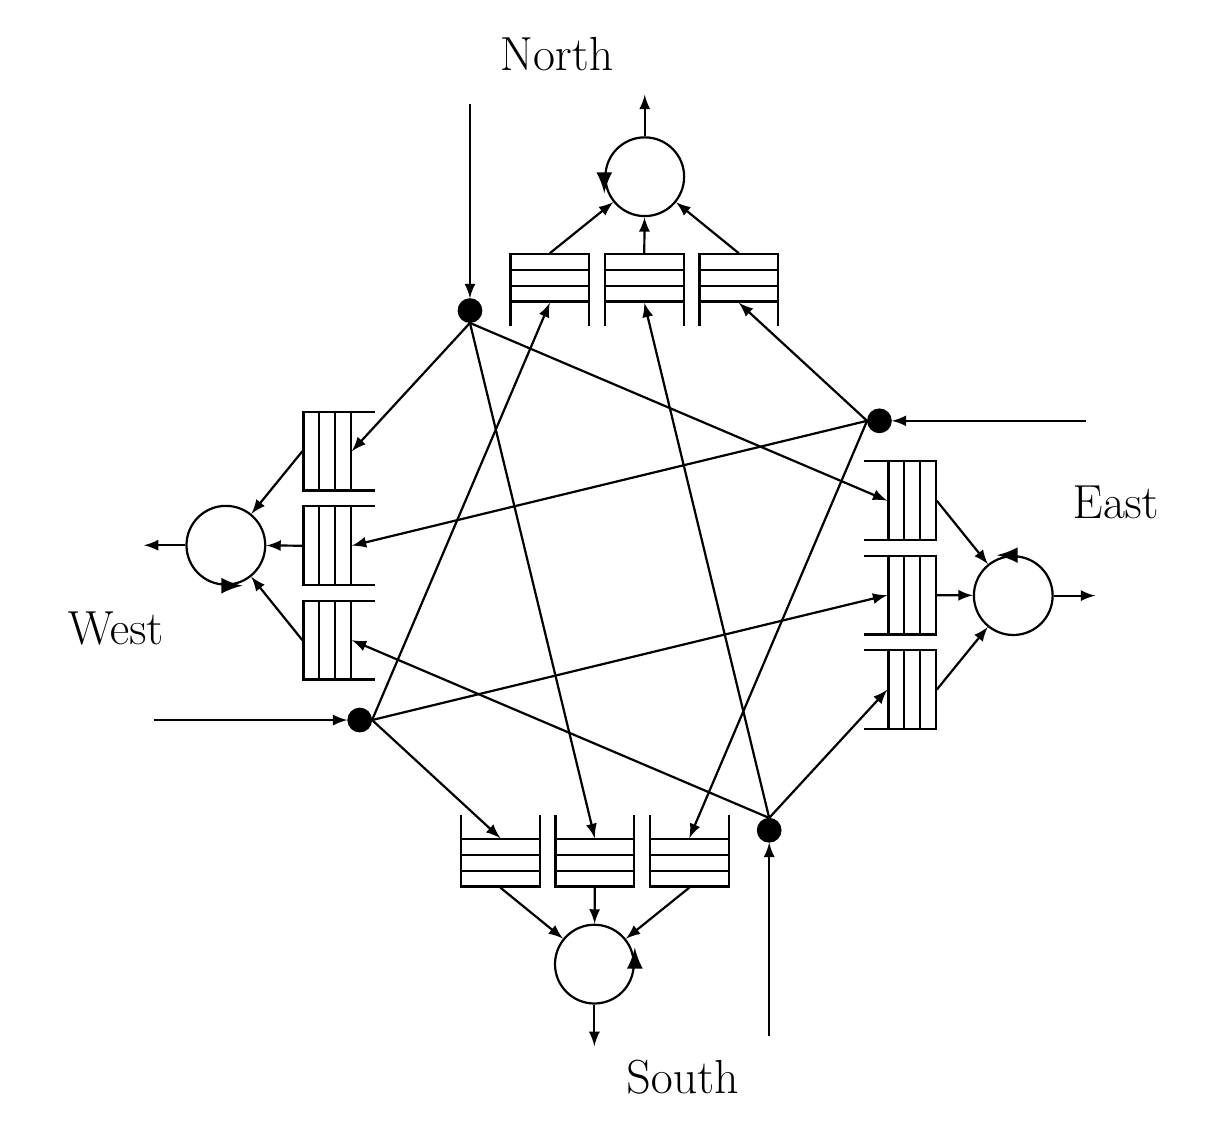
\begin{tikzpicture}[font={\fontsize{12pt}{12}\selectfont}]
    % First, the 4 interfaces
    % North
    \nocswitchint{0}{1}{N}
    % South 
    \begin{scope}[rotate=180, transform shape]
        \nocswitchint{-2.8}{5.8}{S}
    \end{scope}
    % East
    \begin{scope}[rotate=90, transform shape]
        \nocswitchint{-3.8}{2}{E}
    \end{scope}
    % West
    \begin{scope}[rotate=-90, transform shape]
        \nocswitchint{1}{4.8}{W}
    \end{scope}
    
    % Connect the interfaces
    % South -> *
    \draw[thick, ->, >=latex] (rxS.south) -- (buf1n3W.south);
    \draw[thick, ->, >=latex] (rxS.south) -- (buf1n2N.south);
    \draw[thick, ->, >=latex] (rxS.south) -- (buf1n1E.south);
    % West -> *
    \draw[thick, ->, >=latex] (rxW.south) -- (buf1n3N.south);
    \draw[thick, ->, >=latex] (rxW.south) -- (buf1n2E.south);
    \draw[thick, ->, >=latex] (rxW.south) -- (buf1n1S.south);
    % North -> *
    \draw[thick, ->, >=latex] (rxN.south) -- (buf1n3E.south);
    \draw[thick, ->, >=latex] (rxN.south) -- (buf1n2S.south);
    \draw[thick, ->, >=latex] (rxN.south) -- (buf1n1W.south);
    % East -> *
    \draw[thick, ->, >=latex] (rxE.south) -- (buf1n3S.south);
    \draw[thick, ->, >=latex] (rxE.south) -- (buf1n2W.south);
    \draw[thick, ->, >=latex] (rxE.south) -- (buf1n1N.south);
    
    % Interface labels
    \node at (0.6,4.5) [text width=2cm, anchor=north, align=center] {{\LARGE North}};
    \node at (2.2,-8.5) [text width=2cm, anchor=north, align=center] {{\LARGE South}};
    \node at (-5,-2.8) [text width=2cm, anchor=north, align=center] {{\LARGE West}};
    \node at (7.7,-1.2) [text width=2cm, anchor=north, align=center] {{\LARGE East}};
\end{tikzpicture}
